\chapter{Foundation of Logical Normal Form Networks}\label{C:foundation-of-lnfns}
Consider problems with a boolean expression describing the relation ship between binary inputs and outputs. This is certainly a restricted space of problems, however its a logical place to start if defining the activation functions of neurons as a "boolean like" function.\\

With this restriction in place any problem must be described by a boolean expression, this information alone does not help with constructing interpretable networks. It is known that any boolean expression has a CNF and DNF. It is possible to construct networks which can learn the underlying CNF or DNF, such networks are called Logical Normal Form Networks (LNFNs) \cite{herrmann1996backpropagation}. The research developing LNFNs has little justification for key decisions, consequently is difficult to understand and reproduce.\\

Using the idea of LNFNs \cite{herrmann1996backpropagation} and Pure Logical Neural Networks \cite{LearningLogicalActivations} new definitions are given for LNFNs in terms of Noisy-OR and Noisy-AND neurons.

\theoremstyle{definition}
\begin{definition}
A \textbf{CNF-Network} is a three layer network where neurons in the hidden layer consist solely of Noisy-OR's and the output layer is a single Noisy-AND. 
\end{definition}

\theoremstyle{definition}
\begin{definition}
A \textbf{DNF-Network} is a three layer network where neurons in the hidden layer consist solely of Noisy-AND's and the output layer is a single Noisy-OR. 
\end{definition}

\theoremstyle{definition}
\begin{definition}
A \textbf{LNF-Network} is a DNF or CNF Network
\label{def:lnfn}
\end{definition}

A CNF or DNF formula contains clauses of literals which is either an atom or a negation of an atom. To account for this the number of inputs to the network will be doubled, the inputs will be all the atoms and negations of the atoms, i.e. if $x_1, x_2$ are the atoms then $x_1, \lnot x_1, x_2, \lnot x_2$ are the inputs to the network.\\ 

It must also be determined how many hidden units the LNFN will have, it is known that $2^n$, n being the number of atoms, is an upper bound on the number of clauses needed in a CNF and DNF formula (see Theorem \ref{thm:max-clause-cnfdnf}).

\begin{theorem}
Let T be the complete truth table for the boolean formula B. Let L be an LNFN, if L has $2^n$ hidden units then there always exists a set of weights for L which correctly classifies any assignment of truth values to atoms.
\label{thm:upper-bound-hidden-units}
\end{theorem}

\begin{proof}
Let T be the truth table for a boolean function B. The atoms of B are $x_1, ..., x_n$. T has exactly $2^n$ rows. Construct an LNFN, L, in the following manner. L has $2^n$ hidden units and by definition L has one output unit. The inputs to L are $i_1, ..., i_{2n}$ where $i_1, i_2$ represent $x_1, \lnot x_1$ and so on. Let $\epsilon_b = 1$ for every neuron.\\

Let $h_k$ denote hidden unit k. $h_k$ has the weights $\epsilon_{k,1}, ..., \epsilon_{k,2n}$, where $\epsilon_{k, m}$ represents input $i_m$'s relevance to the output of $h_k$. Similarly the output unit $o$ has weights $\mu_1, .., \mu_{2^n}$ where $\mu_m$ represents the relevance of $h_m$ to the output of $o$.\\

Assume L is a DNF Network. Starting from row one of the table T, to row $2^n$. If row $a$ corresponds to False then set $\mu_a = 1$ (i.e. hidden node $a$ is irrelevant), otherwise the row corresponds to True, then $\mu_a = Z$, where Z is a value close to 0 (any weight for a Noisy neuron cant be exactly 0). For each $\epsilon_{a, m}$ if the corresponding literal occurs in row $a$ of the truth table then $\epsilon_{a, m} = Z$ other wise $\epsilon_{a, m} = 1$.\\

\textbf{Claim:} For some assignment to the atoms of B, $x_1 = v_1, ..., x_n = v_n$ where $v_i \in \{0, 1\}$. Then $L(i_1, ..., i_{2n}) = B(x_1, ..., x_n)$.\\

Assume $B(x_1, ..., x_n) = 1$ for the assignment $x_1 = v_1, ..., x_n = v_n$ corresponding to row $a$ of T. Then if $i_k$ is not considered in row $a$ then $\epsilon_{a,k} = 1$ and if it is present then $i_k = 1$. The output of $h_a$ is given by 

\begin{align*}
&= \prod \epsilon_{a, m}^{1 - i_m}\\
&= Z^{\sum_{i_k = 1}(1 - i_k)}\\
&= Z^0
\end{align*}
Demonstrating that  $\lim_{Z \to 0} Out(h_a) = \lim_{Z \to 0} Z^0 = 1$. Consider the activation of $o$, it is known that $\mu_a = Z$ consequently $\lim_{Z \to 0} \mu_a^{h_a} = \lim_{Z \to 0} Z^1 = 0$, therefore

\begin{align}
\lim_{Z \to 0} Out(o) &= 1 - \prod_{m=1}^{2^n} \mu_m ^{h_m}\\
&= 1 - 0 = 1
\end{align} 

Therefore $L(i_1, ..., i_{2n}) = 1$. Alternatively if $B(x_1, ..., x_n) = 0$ then no hidden neuron will have activation $1$, this can be demonstrated by considering that any relevant neuron (i.e. corresponding $\mu \neq 1$) will have some input weight pair of $i_m$ $\epsilon_m$ such that $\epsilon_m^{i_m} = 0$. Consequently it can be said that for all $m$ $\mu_m^{h_m} = \mu_m^{0} = 1$, therefore the output unit will give $0$, as required.

Now assume that L is a CNF Network. The weights can be assigned in the same manner as before, except rather than considering the rows that correspond to True the negation of the rows corresponding to False are used. If a row $a$ corresponds to True then $\mu_a = 1$, otherwise $\mu_a = Z$ and for any literal present in the row then the input to L which corresponds to the negated literal has weight $Z$, all other weights are $1$.\\

\textbf{Claim:} For some assignment to the atoms of B, $x_1 = v_1, ..., x_n = v_n$ where $v_i \in \{0, 1\}$. Then $L(i_1, ..., i_{2n}) = B(x_1, ..., x_n)$.\\

In this configuration it must be shown that every hidden neuron fires when the network is presented with a variable assignment which corresponds to True and there is always at least one neuron which does not fire when the assignment corresponds to False. Assume for a contradiction that for a given assignment $B(x_1, ..., x_n) = 1$ but $L(i_1, ..., i_{2n}) = 0$. Then there is at least one hidden neuron which does not fire. Let $h_a$ be such a neuron. Consequently for any input weight combination which is relevant $\epsilon_{a,m}^{i_m} = 1$, so $i_m = 0$ for any relevant input. Let $i_{r_1}, ..., i_{r_k}$ be the relevant inputs then $i_{r_1} \lor ... \lor i_{r_k} = False$, so $\lnot(\lnot i_{r_1} \land ... \land \lnot i_{r_k}) = False$, a contradiction as then $B(x_1, ..., x_n)$ would be False.

Now assume for a contradiction $B(x_1, ..., x_n) = 0$ but $L(i_1, ..., i_{2n}) = 1$. Then there exists some $h_a$ with output $1$ where it should be $0$. Consequently there exists at least one input/weight pair with $\epsilon_{a,m}^{i_m} = 1$ that should be $0$. Let $i_{r_1}, ..., i_{r_k}$ be all the relevant inputs, at least one relevant input is present $i_r$. Consequently $i_{r_1} \lor ... \lor i_{r_k} = True$, therefore $\lnot(\lnot i_{r_1} \land ... \land \lnot i_{r_k}) = True$, a contradiction as then $B(x_1, ..., x_n)$ is True.\\
\end{proof}

Theorem \ref{thm:upper-bound-hidden-units} provides justification for using $2^n$ hidden units, it guarantees that there at least exists an assignment of weights yielding a network that can correctly classify each item in the truth table.

\section{Noisy Gate Parametrisation} 
The parametrisation of Noisy gates require weight clipping, an expensive operation. A new parametrisation is derived that implicitly clips the weights. Consider that $\epsilon \in (0, 1]$, therefore let $\epsilon_i = \sigma(w_i)$, these $w_i$'s can be trained without any clipping, after training the original $\epsilon_i$'s can be recovered.\\

Now these weights must be substituted into the Noisy activation. Consider the Noisy-OR activation.

\begin{align*}
a_{or}(X) &= 1 - \prod^p_{i=1}(\epsilon_i^{x_i}) \cdot \epsilon_b\\
&= 1 - \prod^p_{i=1}(\sigma(w_i)^{x_i}) \cdot \sigma(b)\\
&= 1 - \prod^p_{i=1}((\frac{1}{1 + e^{-w_i}})^{x_i}) \cdot \frac{1}{1 + e^{-b}}\\
&= 1 - \prod^p_{i=1}((1 + e^{-w_i})^{-x_i}) \cdot (1 + e^{-w_i})^{-1}\\
&= 1 - e^{\sum^p_{i=1} -x_i \cdot ln(1 + e^{-w_i}) - ln(1 + e^{-b})} \\
&Let\ w_i^{'} = ln(1 + e^{-w_i}),\ b^{'} = ln(1 + e^{-b})\\
&= 1 - e^{-(W^{'} \cdot X + b^{'})}
\end{align*}

From a similar derivation we get the activation for a Noisy-AND.

\begin{align*}
a_{and}(X) &= \prod_{p}^{i=1} (\epsilon_i^{1 - x_i}) \cdot \epsilon_b\\
&= \prod_{p}^{i=1} (\sigma(w_i)^{1 - x_i}) \cdot \sigma(w_b)\\
&= e^{\sum^p_{i=1} -(1 - x_i) \cdot ln(1 + e^{-w_i}) - ln(1 + e^{-b})} \\
&= e^{-(W^{'} \cdot (1 - X) + b^{'})}
\end{align*}

Concisely giving equations \ref{equ:real-noisy-and-activation}, \ref{equ:real-noisy-or-activation}

\begin{align}
a_{and}(X) &= e^{-(W^{'} \cdot (1 - X) + b^{'})} \label{equ:real-noisy-and-activation}\\
a_{or}(X)&= 1 - e^{-(W^{'} \cdot X + b^{'})} \label{equ:real-noisy-or-activation}
\end{align}

The function taking $w_i$ to $w_i^{'}$ is the soft ReLU function which is performing a soft clipping on the $w_i$'s. 

\section{Training LNF Networks}
Using equations \ref{equ:real-noisy-or-activation} and \ref{equ:real-noisy-and-activation} for the Noisy-OR, Noisy-AND activations retrospectively allows LNFNs to be trained without the need to clip the weights.\\

Training the networks on all input patterns at the same time lead to poor learning, whereas training on a single example at a time had significantly better results. The ADAM Optimizer is the learning algorithm used, firstly for the convenience of an adaptive learning rate but also because it includes the advantages of RMSProp which works well with on-line (single-example) learning \cite{kingma2014adam}, which LNFNs respond well to.\\

Preliminary testing showed that LNFN's are able to learn good classifiers on boolean gates, i.e. NOT, AND, NOR, NAND, XOR and Implies. It is also possible to inspect the trained weights and see that the networks have learnt the correct CNF or DNF representation.

\section{LNF Network Performance}
How do LNFNs perform against standard perceptron networks which we know to be universal function approximators. Two different perceptron networks will be used as a benchmark

\begin{enumerate}
	\item One will have the same configuration as the LNFNs, i.e. $2^n$ hidden neurons.
	\item The other has two hidden layers, both with N neurons.
\end{enumerate}

The testing will consist of selecting 5 random boolean expressions for $2 \leq n \leq 9$ and training each network 5 times, each with random initial conditions. Figure \ref{fig:peformance-comparason-all} shows a comparison between all 4 of the networks and figure \ref{fig:peformance-comparason-cnfdnf} shows just the LNFN's.

\begin{figure}[H]
  \centering
  \begin{minipage}[b]{0.8\textwidth}
    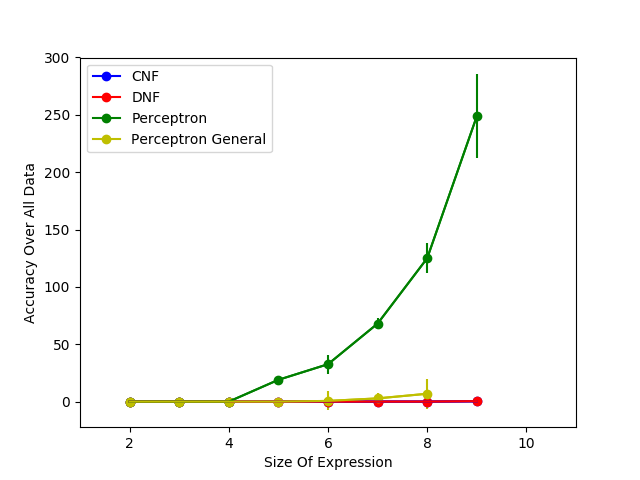
\includegraphics[width=\textwidth]{All-Peformance-Comparason.png}
    \caption{}
    \label{fig:peformance-comparason-all}
  \end{minipage}
  \hfill
\end{figure}

\begin{figure}[H]
  \centering
  \begin{minipage}[b]{0.8\textwidth}
    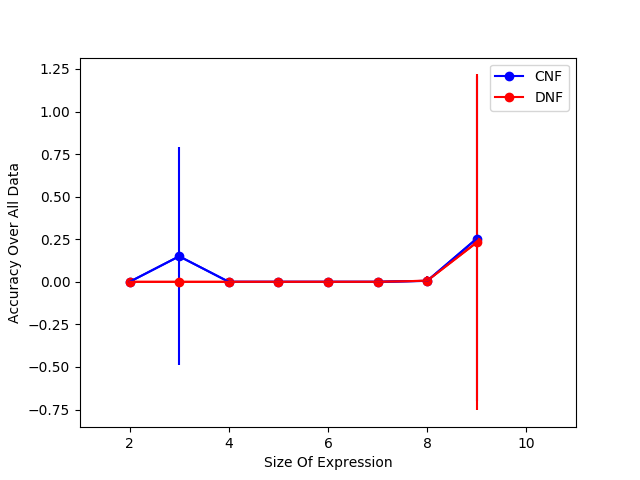
\includegraphics[width=\textwidth]{CNFvsDNF.png}
    \caption{}
    \label{fig:peformance-comparason-cnfdnf}
  \end{minipage}
  \hfill
\end{figure}

Figure  \ref{fig:peformance-comparason-all} shows that neither of the perceptron networks perform as well as the LNF Networks as $n$ increases. Figure  \ref{fig:peformance-comparason-cnfdnf} shows on average there are no statistically significant differences between the CNF or DNF networks. What is not present in Figure \ref{fig:peformance-comparason-cnfdnf} is that sometimes the CNF network consistently out performs the DNF and visa versa, theoretically both should be able to learn any boolean expression.

What causes some expressions to be harder to learn for one type of LNFN compared to another? 

\section{LNF Network Generalization} \label{sec:lnfn-generalization}
These networks are able to perform as well as standard perceptron networks but so far they have been getting the complete set of data, in practice this will almost never be the case. Standard ANN's are widely used because of their ability to generalize, for LNFN's to be useful they must also be able to generalize.

\begin{figure}[H]
	\centering
	\begin{minipage}[b]{0.8\textwidth}
		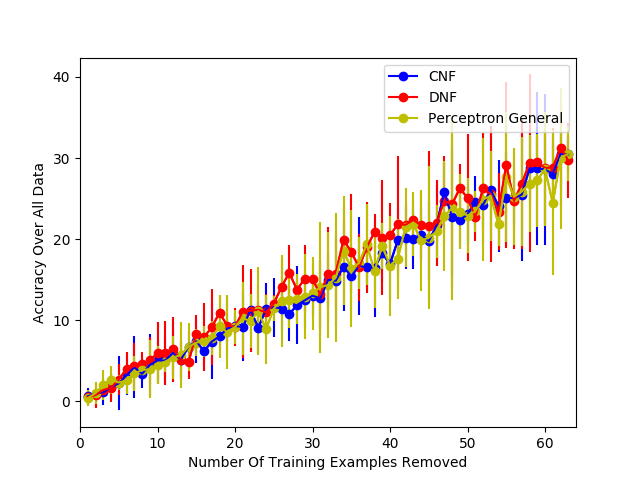
\includegraphics[width=\textwidth]{6-generalization.png}
		\caption{}
		\label{fig:generalization-peformance-6}
	\end{minipage}
	\hfill
\end{figure}

Figure \ref{fig:generalization-peformance-6} shows a comparison between the generalization ability of CNF, DNF and Perceptron networks. The graph shows the performance over all training data when successively removing elements from the training set. It demonstrates that the CNF and DNF networks generalize as well as the perceptron networks when the boolean formula has 6 inputs, this trend continues as n increases up to 9.

\section{LNF Network Rule Extraction}
Given the logical nature of LNFNs, is it possible to extract boolean rules. Consider the weights for a logical neuron $W = \{w_1, ..., w_n\}$, These can be converted to $\epsilon_i = \sigma(w_i)$ where $\epsilon_i \in [0, 1]$ and represents the relevance input $x_i$ has on the neurons output.\\

To extract meaningful rules from the network using $\{ \epsilon_1, ..., \epsilon_n \}$ it is important that at the conclusion of training each $\epsilon_i \approxeq 1$ or $\epsilon_i \approxeq 0$. If this is the case then it is possible to interpret the neuron as a purely logical function, say that the neuron in question was a Noisy-OR, then the neuron can be seen as performing a logical OR on all the inputs with corresponding $\epsilon \approxeq 0$.\\

Conjecture \ref{conj:lnfn-approach-binary} is the foundation of the following rule extraction algorithm, it was derived from experimental evidence by training LNFNs over complete truth tables and inspecting the weights. Ideally Conjecture \ref{conj:lnfn-approach-binary} would be proved, but that is out of scope for this report.

\begin{conjecture}
	For an LNFN network trained on a binary classification problem with boolean inputs, as the loss approaches 0  (i.e. the correct CNF or DNF has been found) the weights $\{ w_1, ..., w_n \}$ approach $\infty$ or $-\infty$, consequently each $\epsilon_i$ approaches 0 or 1.
	\label{conj:lnfn-approach-binary}
\end{conjecture}

The Algorithm displayed in figure \ref{alg:rule-extraction} extracts rules from CNFNs, it takes the output weights (ow) and hidden weights (hw) as input and outputs the a boolean expression. A similar algorithm can be derived for DNFNs, it is omitted but can be obtained by simply switching the logical operations around.

\begin{figure}[H]
	\begin{lstlisting}[mathescape=true]
atoms = $\{ x_1, \lnot x_1, ... x_n, \lnot x_n, \}$
	
function extractRulesCNFN(ow, hw)
  ow $= \sigma($ow$)$
  hw $= \sigma($hw$)$
  relvHidden = [hw[i] where ow[i] := 0]
		
  and = And([])
    for weights in relvHidden
      or = Or([atoms[i] where weights[i] := 0])
      and.add(or)
		
  return and
	\end{lstlisting}
	\caption{Rule Extraction Algorithm (for CNFN)}
	\label{alg:rule-extraction}
\end{figure}

In practice many clauses in the extracted expression contain redundant terms, i.e. clauses that are a tautology or a duplicate of another, filtering these out is not an expensive operation.\\

Section \ref{sec:lnfn-generalization} discusses the generalization capabilities of LNFNs compared to MLPNs and shows that they are statistically equivalent. How does training over incomplete truth tables effect the generalization of extracted rules and what factors could influence this?\\

Consider $B$ to be the set of all boolean problems with $n$ inputs. What is the cardinality of $B$, there are $2^n$ rows in the truth table and $2^{2^n}$ ways to assign true/false values to these rows, each way corresponding to a different boolean function, consequently $|B| = 2^{2^n}$. So consider some $b \in B$ represented by $2^n$ rows of a truth table, removing one row from the training data means there are now two possible functions that could be learnt, one where the removed row corresponds to true and the other to false. As more rows are removed this problem is compounded, if $m$ rows are taken then there are $2^m$ possible functions.\\

When constructing a CNF or DNF from a truth table as discussed in Section \ref{subsec:construct-cnfdnf}, in the case of CNF only the rows corresponding to false are considered and for the DNF only rows corresponding to true. Despite the fact that if $m$ rows are removed from the training set then there are $2^m$ possible functions that could represent the partial truth table, learning the CNF and DNF may alleviate some of the issues caused by it, another possibility is to combine the CNF and DNF formulas to create a better rule set.\\

Figure \ref{fig:cnf-descrete-generalizatiion} shows how the rule set of an CNFN generalizes as examples are removed, figure \ref{fig:dnf-descrete-generalizatiion} shows the same but for DNFNs.

\begin{figure}[H]
	\centering
	\begin{minipage}[b]{0.45\textwidth}
		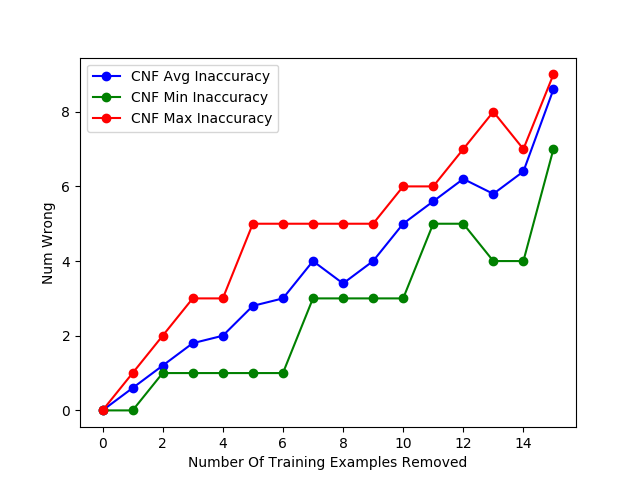
\includegraphics[width=\textwidth]{cnf-descrete-generalization.png}
		\caption{}
		\label{fig:cnf-descrete-generalizatiion}
	\end{minipage}
	\begin{minipage}[b]{0.45\textwidth}
		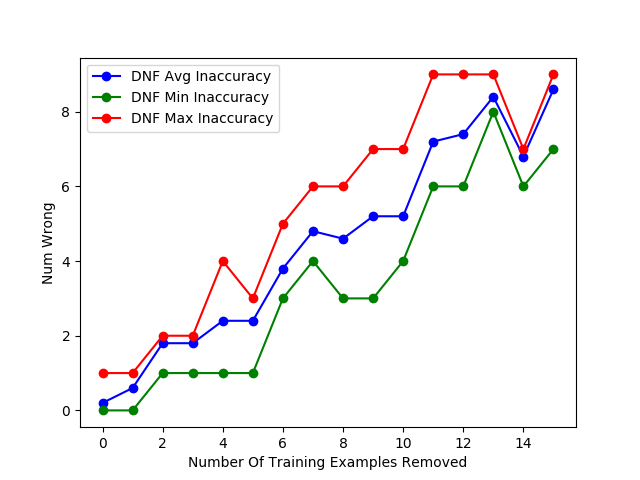
\includegraphics[width=\textwidth]{dnf-descrete-generalization.png}
		\caption{}
		\label{fig:dnf-descrete-generalizatiion}
	\end{minipage}
	\hfill
\end{figure}

In figures \ref{fig:cnf-descrete-generalizatiion} \& \ref{fig:dnf-descrete-generalizatiion} the training examples which are removed get randomly selected, how is the performance effected if the removed examples are chosen more carefully. In the next experiment only examples corresponding to false are removed and the resultant training set is given to a DNFN.

\begin{figure}[H]
	\centering
	\begin{minipage}[b]{0.45\textwidth}
		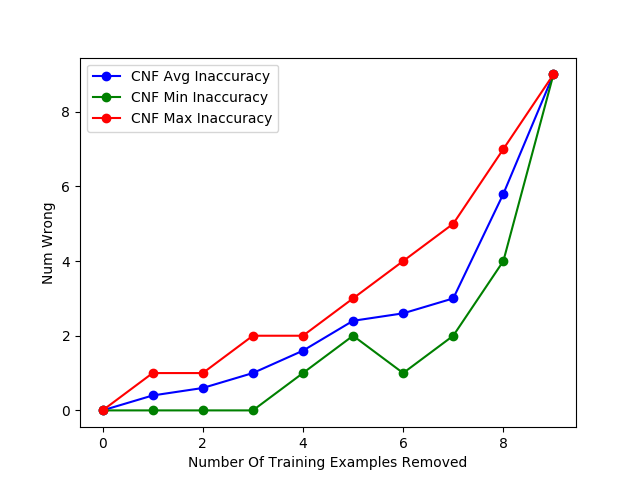
\includegraphics[width=\textwidth]{cnf-descrete-generalization-partial.png}
		\caption{}
		\label{fig:cnf-descrete-generalizatiion-partial}
	\end{minipage}
	\begin{minipage}[b]{0.45\textwidth}
		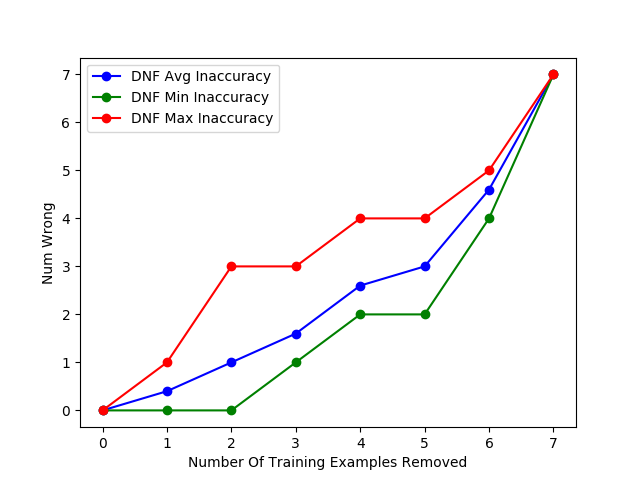
\includegraphics[width=\textwidth]{dnf-descrete-generalization-partial.png}
		\caption{}
		\label{fig:dnf-descrete-generalizatiion-partial}
	\end{minipage}
	\hfill
\end{figure}

Figures \ref{fig:cnf-descrete-generalizatiion-partial} \& \ref{fig:dnf-descrete-generalizatiion-partial} demontrait CNFNs and DNFNs trainined over partial data retrospectively. In the case of CNFNs only true entries of the truth table are removed and for the DNFNs only false entries. For the most part the minimum line is lower however the average line is roughly the same, this would indicate that initial conditions have an effect on the generalization performance.

\chapter{Investigation of Logical Normal Form Networks} \label{C:investigation-of-lnfns}
\section{Developing Applications} \label{sec:developing-applications}
The LNFNs presented in Chapter \ref{C:foundation-of-lnfns} have very limited applications, the class of problems they can be applied to all have the form of binary classification where the features are Boolean. To make LNFNs more useful they need a broader scope.

\subsection{Multi-class Classification}
How can LNFNs be developed] to support classification of more than two classes. If attempting to learn a Multi-class Classification problem with $n$ distinct classes $c_1, ..., c_n$, then $n$ LNFNs would have to be trained, each a learning a binary classification problem $c_i$, $\lnot c_i$.\\

An intuitive way to extend LNFNs to support Multi-class Classification is to add more output neurons and use One-hot encoding. If we have 3 classes then $100$, $010$ and $001$ represent class 1, 2 and 3 retrospectively, then the LNFN would have 3 output neurons, each representing a bit in the One-hot encoded string.\\

\begin{definition}
	The structure of an LNFN to solve an $k$ class classification problem where each instance is described by n features has $2n$ inputs, $2^n$ hidden units and $k$ output units. A final Softmax layer is added, as is convention for these types of problems.
\end{definition}

A simple problem which lends its self naturally to this is the \text{Lenses} problem \cite{Lichman:2013}, a three class classification problem, each instance has 4 features, 3 of which are binary and the other has three possible values. This problem can be easily converted into one which can be used with an LNFN, each new problem instance will have 6 features, the three binary remain the same and the categorical one is expanded into 3.\\

How does an LNFN network perform when compared to a MLPN on the Lenses problem. The performance of the two classifiers will be compared using Leave-One-Out (LOE) Cross-Validation. The structure of the MLPN only differs in the number of hidden layers/units, there are two hidden layers, one with $2 \cdot n$ hidden units and the other with $n$

\begin{table}[H]
	\begin{center}
		\begin{tabular}{| c | c | c |}
			\hline
			& Error (Cross Entropy) & Confidence Interval (95\%) \\
			\hline
			CNF Net & 6.663 & (6.468, 7.198) \\
			\hline
			DNF Net & 6.660 & (6.468, 7.197) \\
			\hline
			PCEP Net & 6.751 & (6.468, 7.997) \\
			\hline
		\end{tabular}
	\end{center}
	\caption{}
	\label{tab:lenses-peformance-comp}
\end{table}

Table \ref{tab:lenses-peformance-comp} demonstrates that the CNF \& DNF Networks perform comparably to an MLPN as the confidence intervals for the error overlap.\\ 

Now that the LNFN network has three output neurons it should be possible to extract three rules describing each of the classes. Consider that each problem instance is of the following form $\{a, b, c, d, e, f\}$ where $a,b,c,d,e,f$ are all atoms. The following rules can be extracted from a CNFN when trained over the complete Lenses data, any duplicate clause or Tautology has been filtered out, the resultant extracted formula has also been manually simplified (so they can be displayed and understood better).

\begin{itemize}
	\item \text{Class 1:} $(a \lor b \lor e) \land (a \lor \lnot d) \land (c \lor e) \land f$
	\item \text{Class 2:} $(a \lor b \lor \lnot c \lor d) \land \lnot e \land f$
	\item \text{Class 3:} $(\lnot a \lor b \lor c \lor \lnot f) \land (a \lor \lnot d \lor e \lor \lnot f) \land (\lnot b \lor c \lor d \lor \lnot f) \land (d \lor \lnot e \lor \lnot f)$
\end{itemize}

Immediately it is possible to find useful information about this problem that was not obvious before, namely $\lnot f = True \implies $ Class 3. Table \ref{tab:rule-classification-lenses-cnf} shows these rules applied to all the problem instances in the Lenses data set, it demonstrates that these extracted rules are able to fully describe the Lenses problem.\\

The DNFN might be more applicable as the rules will be more insightful, given its structure as an OR of ANDs.\\

\begin{itemize}
	\item \text{Class 1:} $(a \land \lnot b \land \lnot c \land e \land f) \lor (\lnot a \land \lnot d \land e \land f)$
	\item \text{Class 2:} $(\lnot c \land \lnot e \land f) \lor (c \land d \land \lnot e \land f)$
	\item \text{Class 3:} $(\lnot a \land \lnot b \land c \land \lnot d) \lor (\lnot a \land d \land e) \lor \lnot f$
\end{itemize}

These DNF formula do not correspond to the CNF give above but this is to be expected, despite the fact that collectivity all the problem instances span the space of features once they have been converted to the boolean feature form this fact is no longer true.    there is a way to combine the knowledge from both the CNF and DNF formula to create resultant formula which perform better.\\

One possible issue that could arrive here is that the CNFN is now attempting to learn three CNF expressions with the same number of hidden neurons. The fact that meaningful rules where able to be extracted in this case could of been a coincidence, intuitively if we are learning a problem with $k$ classes then we could need $k \cdot 2^n$ hidden neurons which is becoming impractical.

\subsection{Features with Continuous Domains}
The inputs to an LNFN are allowed to be continuous but must be in the rage $[0, 1]$, would it still be possible to extract meaningful rules from the network if the inputs are continuous? Here there are two things to investigate. What can be achieved by training an LNFN on problems with continuous features? Secondly what can be achieved by discretizing the continuous inputs and then using an LNFN to learn this new boolean problem. A simple benchmark to use is the Iris problem \cite{Lichman:2013}

\subsubsection{LNFNs and Continuous Features} \label{subsubsec:lnfns-cont-features}
If the features are continuous it no longer makes sense to extract rules but it could still be possible to see what inputs are considered in making a decision about the class. When training an LNFN on the Iris problem (over all problem instances) the network converges to a solution with a loss of $96.932$, poor performance when compared to a perceptron network that can achieve an accuracy of $0.0$. \\

Inspecting the class prediction of each reveals that for a problem instance that has a true class of Iris-virginica or Iris-versicolor then LNFN sometimes predicts multiple classes, this leads to the belief that these networks have issues with learning problems that are not linearly separable as the two classes which an LNFN has trouble differentiating between are not linearly separable.\\

The LNFN is able to learn XOR so not all problems which are not linearly separable are out of reach of LNFNs. Section \ref{subsubsec:lnfns-desc-cont-features} investigates whether it is possible to descretize the variables in such a way that makes this problem learnable by LNFNs.


\subsubsection{LNFNs and Discretized Continuous Features} \label{subsubsec:lnfns-desc-cont-features}
There are a number of method for discretizing continuous features, there are many algorithms for performing such an operation on some data \cite{liu2002discretization}, to many for all to be tested. Two simple methods for descretization are Equal width or frequency binning, these methods are very naive and prone to outliers, also the number of bins must be chosen before hand so this requires experimentation. A supervised partitioning method will also be tested, namely Recursive Minimal Entropy Partitioning.\\

Results from training LNFNs with descretized data results in the same issue as before, the network has problems with classifying classes that are not linearly separable.

\subsubsection{Discussion of Application to Continuous Domains}
The ideas explored in Sections \ref{subsubsec:lnfns-cont-features} \& \ref{subsubsec:lnfns-desc-cont-features} demonstrate that applying LNFNs to problems with continuous inputs is not viable.


\section{Evaluation of LNFN Intepretability}
LNFNs are more interpretable than standard MLPNs, demonstrated by the ability to directly extract rules from the neurons by observing the weights. Being able to understand LNFNs comes at a cost of reducing the functions which they can approximate, as shown in Section \ref{sec:developing-applications}. How does the information extracted from LNFNs compare to the rules which can be obtained from MLPNs using existing techniques?

\subsection{Evaluation of LNFN Rules}

\subsection{Comparason Between Rules from LNFNs and MLPNs}
To determine the usefulness of LNFNs and the rules which can be extracted from them a comparison to existing methods must be preformed. The rules extracted from MLPNs will be compared to thoughs from LNFNs.

\chapter{Logical Neural Networks}
The algorythm shown in Figure \ref{alg:rule-extraction} presents a method for extracting rules from LNFNs, there is no reason why this algorithm cant be applied to Logical Neural Networks (LNNs) \cite{LearningLogicalActivations} which can take on any configuration.\\

An issue with LNFNs is that the number of hidden units allows for the possibility to memorise the input data, using LNNs consisting of more layers with a smaller width could force the learning of better rules.\\

Before investigating this there are two key issues caused by removing the restrictions imposed by the LNFN definition (Definition \ref{def:lnfn}) which must be addressed 

\begin{enumerate}
	\item Noisy neurons do not have the capacity to consider the presence of the negation of an input. This was a problem for LNFNs as well, however given that only the negations of atoms need to be considered to learn a CNF or DNF it was easily fixed by presenting the network with each atom and its negation. The problem can not be solved so easily for LNNs. A boolean formula can not always be represented by only AND and OR gate, i.e the set of operations $\{AND, OR\}$ is not functionally complete. 
	
	\item Another problem faced by LLNs that are not restricted to be ether a CNFN or DNFN is that the structure of the network will have a higher impact on whether the problem can be learnt. 
\end{enumerate}

Despite the issues outlined above being able to implement LNNs with layers that are not required to be $2^n$ hidden units wide would be alot more practical, in practice the number of features could be upwards of 100 and $2^100$ is a huge number of hidden neurons.\\

Resolving Issue 1 involves making our operation set functionally complete, this requires the $NOT$ operation. There are two ways to include the $NOT$ operation in the LNNs, one is to simply perform the augment the inputs to each layer to include each input and its negation, a more complicated but more elegant solution is to derive a parametrisation of Noisy gates which can learn to negate inputs.